%\documentclass[10pts, twocolumn]{article}
%\documentclass[twocolumn]{IEEEtran}
\documentclass[final]{ieee}
\usepackage { graphicx}
\usepackage{wrapfig}

\hyphenation{librar-ian librar-ians shep-herd bar-tender gate-way name-space}

\begin{document}
\pagestyle{headings} 
\title{Service-Oriented ARC Storage; \\An Overview and Design}
%% \author{  Jon K. Nilsen$^{2,3}$ \and Salman Toor$^{1}$
%%   \and Zsombor Nagy$^{5}$ \and Bjarte Mohn$^{4}$  \\ $^{1}$Scientific
%%   Computing Division, IT Department, Uppsala University, Sweden
%%   \\ $^{2}$Center for Information Technology, University of Oslo, Norway
%%   \\ $^{3}$Department of Physics,  University of Oslo, Norway
%%   \\  $^{4}$Department of Physics and Astronomy, Uppsala University,
%%   Sweden \\ $^{5}$National Information Infrastructure Development
%%   Institute, Hungary}
\author{  Jon K. Nilsen$^{\dagger,\ddagger}$ \and Salman Toor$^{*}$
  \and Zsombor Nagy$^{\mathparagraph}$ \and Bjarte Mohn$^{\mathsection}$ 
\\$^{*}$Dept. of Information Technology, Div. of Scientific Computing, Uppsala
University,\\ Box~337, SE-75105~Uppsala, Sweden
 \\ $^{\dagger}$University of Oslo, Center for Information Technology,\\
P.~O.~Box~1059, Blindern, N-0316~Oslo, Norway
  \\ $^{\ddagger}$University of Oslo, Dept. of Physics, P.~O.~Box~1048,
Blindern, N-0316~Oslo, Norway
  \\  $^{\mathsection}$Dept. of Physics and Astronomy, Div. of Nuclear and
Particle Physics,\\ Uppsala University, Box~535, SE-75121~Uppsala, Sweden \\
$^{\mathparagraph}$Institute of National Information and Infrastructure
Development\\ NIIF/HUNGARNET, Victor~Hugo~18-22, H-1132~Budapest, Hungary\\ \\ 
j.k.nilsen@usit.uio.no \hspace{5 mm}
  salman.toor@it.uu.se \hspace{5 mm} zsombor@niif.hu \\  \hspace{7 mm}
  bjarte.mohn@fysast.uu.se}
  
  % \\ \small{salman.toor \and bjarte.mohn  }}

\maketitle             
%% \begin{abstract}
%% The KnowARC project will deliver the next generation Advanced Resource
%% Connector Fall  2009. A major component of this
%% service-oriented Grid middleware will be its storage system, the
%% ARC Storage, of which a
%% prototype is due Spring 2009. We will in this paper present an
%% overview of the storage system, its design and architecture. We will
%% also present some first, proof-of-concept test results, deploying the
%% the storage with a geographically distribution among three different countries.
%% ~\\~\\~
%% \end{abstract}
\begin{abstract}
There is an ever increasing need to utilize geographically distributed
hardware resources, both in terms of CPU and in terms of storage. The
service-oriented architecture provides a natural framework for
managing these resources. The next generation Advanced Resource
Connector (ARC) is a service-oriented Grid solution that will provide
the middleware to represent distributed resources in one simple
framework. In this paper, we will present an overview of the ARC
storage system, itself a set of services providing a self-healing,
flexible Grid storage solution. We will also present some first
proof-of-concept test results from a deployment of the storage system
distributed across three different countries. 
~\\~\\~
\end{abstract}
%-----------------------------------------------------------
\section{Introduction}
\label{Introduction}

The challenge of building a reliable, self-healing, fault-tolerant,
consistent data management system at the web-scale is an interesting
task. Making the system work in a heterogeneous, distributed
environment like the Grid is even more interesting. An increasing
number of applications demand not only increased CPU power, but also
vast amounts of storage space. The required storage space is not only
restricted to the duration in which the application runs; the data
should often be available for years afterwards, in certain cases even
for decades. Nowadays, we can easily find single Grid jobs which produce
gigabytes or even terabytes of data, ramping up the requirements of
storage systems to the petabyte-scale and beyond. Hard drive capacity is
still increasing and storage raids can handle failing hard drives through 
data replication. However, even a designated storage site cannot guarantee 
24/7 availability or long-term security against catastrophic losses of data. 
The need for a distributed, self-healing storage system is evident. To
make the storage system useable to Grid users, the system must provide
reliable and secure file transfer protocols, a cataloging system and
secure storage of the data. Several projects and designs have emerged
to address such challenges~\cite{Hoschek00datamanagement,DengWang}.

In the advent of the next generation of the Advanced Resource
Connector (ARC) Grid middleware~\cite{arc} (new release due during
fall 2009), we present the ARC storage
system~\cite{ARCStoragedesigndoc}. This distributed storage system is
designed to provide an easy to use, flexible and scalable system that
can offer native storage and at the same time provide access to
third-party solutions like dCache~\cite{dCache,DSSWithdCache} by using
the same, uniform interface. Being part of ARC, the storage system is
based on a service-oriented architecture, in which each major
component of the system runs as a separate service within the ARC
Hosting Environment Daemon (HED)~\cite{HEDdesigndoc}. The HED service
container gives the capability of flexible replacement of the
components as well as the possibility to introduce modifications in
the future. %% The HED service container gives
%% the capability of flexible replacement of the components as well as
%% the future modification/enhancement of the system.

This paper is organized as follows. After describing
related work in Section \ref{Related Work}, we give a bird's eye
view of the next-generation Advanced Resource Connector (ARC) in
Section \ref{The Advance Resource Connector}. An overview of the
ARC Storage is given in Section \ref{The ARC Storage System}, while
the architecture of the storage system is elaborated in Section
\ref{Architecture of the ARC Storage}. In Section \ref{Testing and
  Discussion} we give some early, proof-of-concept results, before 
concluding in Section \ref{Conclusion and Future Work}. 

\section{Related Work}
\label{Related Work}
\textbf{dCache:} dCache is a storage system which combines heterogeneous storage
elements to collect several hundreds of terabytes in a single
namespace. It additionally supports standard and native
protocols like gridftp, srm, dcap and gsidcap. dCache is
a joint effort between DESY \cite{dCachesite}, Fermi National Accelerator Laboratory \cite{FermiLab}, the  Nordic Data
Grid Facility (NDGF) \cite{NDGF}  and several other collaborators. %% The services or
%% components of dCache are known as cells. The standard deployment of
%% dCache consist of  storage pools; used to store file, optionally be
%% connected with HSM\footnote{Hierarchical Storage Manager, used for the
%%   tape storage}. Namespace manager; used PNFS \footnote{Perfectly
%%   Normal FileSystem; A network file system, designed in Desy} as a
%% filesystem  for storing matadata. And the number of protocol
%% doors. One of the biggest deployment of dCache is the distributed
%% infrastructure of  NDGF.\\ 
dCache has proven to be a very stable and scalable solution. However,
it is relatively difficult to deploy and integrate with new applications. 
The ARC Storage, being a light-weight and flexible
storage solution, aims more towards new user groups less familiar with
Grid solutions. 
\newline
\textbf{BigTable:} Bigtable is a distributed storage system managing structured data on
the petabyte-scale \cite{Bigtable}. It is currently used within
Google in projects such as web indexing, Google Earth and Google
Financing. %% Bigtable is mainly built on top of three pieces of Google's
%% infrastructure: The Google Filesystem \cite{GFS} a distributed,
%% replicating file system, the Google SSTable, providing
%% a persistent, ordered immutable map and Chubby \cite{Chubby}, a highly
%% available and persistent distributed lock service. The system uses a
%% three-level B$^+$-tree to store \textit{tablets}. The location of the
%% first level is stored in Chubby, making Chubby a vitaly important part
%% of the design. To ensure a persistent solution, Chubby takes advantage
%% of the Paxos algorithm \cite{Paxos,PaxosLive}.\\
Bigtable has several interesting features, one of which is the
distributed lock service, Chubby \cite{Chubby}. Chubby is a high-availability, distributed
locking service sitting on top of the B$^+$-tree architecture of
Bigtable. Chubby has several features similar to our A-Hash service (see Section \ref{Hash Algorithm}),
among which the use of the Paxos algorithm \cite{Paxos,PaxosLive}, is
the most striking. A major caveat for the Grid community is that
Bigtable is neither free, open-source nor available to the public.
\newline
\textbf{Storage Resource Broker:}  Based on the client-server model,
the Storage Resource Broker (SRB) \cite{earlySRB,SRB} provides a flexible data grid management
system. It allows  uniform access to heterogeneous
storage resources over a wide area network. %% SRB also manages the
%% namespaces used to identify files, storage resources, users, metadata,
%% and access controls independently of the physical storage systems. It
%% uses centralized matadata catalog (MCat). Also supports several file
%% systems of UNIX, Windows, Linux, Mac OS X, HPSS and large scale
%% storage systems like Castor and dCache.\\
Its functionality, with a uniform namespace for several Data Grid
Managers and file systems, is quite similar to the functionality
offered by our Gateway service (see Section \ref{Gateways}). However, being built as a middleware on top of
other major storage solutions, SRB does not offer its own storage solution.
\newline
\textbf{Scalla:} Scalla is a widely used software suite consisting of an
xrootd server for data access, and an olbd
server for building scalable xrootd clusters \cite{Scalla}. %% The xrootd
%% server consists of several plug-in based components, of which the most
%% important are; the xrd component, responsible for network, threading,
%% data buffer and protocol management; the xroot protocol component,
%% providing the specialized and increasingly popular xroot protocol; and
%% components for logical and physical file systems. The olbd server is
%% used for setting up storage clusters in a B-64 tree with a
%% redirector on top appointing one supervisor for every 64 data servers
%% in the lower layers of the tree.
Originally developed for use with the physics analysis tool root \cite{root},
xrootd offers data access both through the specialized xroot protocol
and through other third-party protocols. The combination of the xrootd
and olbd components offers a cluster storage designed for low latency,
high bandwidth environments. In contrast, ARC Storage is optimized
for high latency and is more suitable for the Grid environment.

%% {\large Comparison:}    

%% dCache is a very scalable solution, but it has a relatively high
%% threshold (more under standing is required) for learning and
%% deployment.  Proposed solution is more light-weight, flexible and
%% hence more suitable for the new users.  

%% Xrootd with OBLD is a cluster storage designed for low latency high
%% bandwidth. Our solution is optimized for high latency more suitable
%% for Grid environment. 

%% Big table can handle extreme amount  of data and vast number of
%% users. How ever it is still an in-house solution.  

%% The functionality of SRB, where there is a uniform namespace for
%% several DGMS and file systems, is very similar to our gateway service.    



\section{The Advanced Resource Connector}
\label{The Advance Resource Connector}

The next generation of Advanced Resource Connector (ARC) Grid middleware is
developed by NorduGrid~\cite{NorduGridsite} and the EU KnowARC
 project~\cite{KnowARCsite}. It consists of a set of pluggable 
components. These components are the
fundamental building blocks of the ARC services and clients. ARC
services run inside a container called the Hosting Environment
Daemon (HED) and there are four kinds of pluggable components with well
defined tasks: Data Management Components are used to transfer the
data using various protocols, Message Chain Components are
responsible for the communication within clients and services as well as
between the clients and the services, ARC Client Components are
plug-ins used by the clients to connect to different Grid flavors, and
Policy Decision Components are responsible for the security model
within the system.

To deliver the non-trivial quality of services required by the Grid,
there are a number of services running inside the HED. For example, Grid
job execution and management is handled by the A-REX service 
\cite{AREXdesigndoc}, policy
decisions are taken by the Charon service, the ISIS service is
responsible for information indexing, batch job submission is
handled by the Sched service, etc. In the later sections our discussion
will focus on the architecture and the design of another major set
of services, i.e., the ARC storage. 

\section{The ARC Storage System}
\label{The ARC Storage System}

The ARC Storage consists of a set of SOAP based services residing
within HED. Together, the services provide a self-healing, reliable, robust,
scalable, resilient and consistent data storage system. Data is
managed in a hierarchical global namespace with files and
subcollections grouped into collections\footnote{A concept very
  similar to files and directories in most common file systems.}.  A
dedicated root collection serves as a reference point for accessing the namespace. The hierarchy can then be
referenced using Logical Names. The global namespace is accessed
in the same manner as in local filesystems.

\begin{figure}
  \begin{center}
    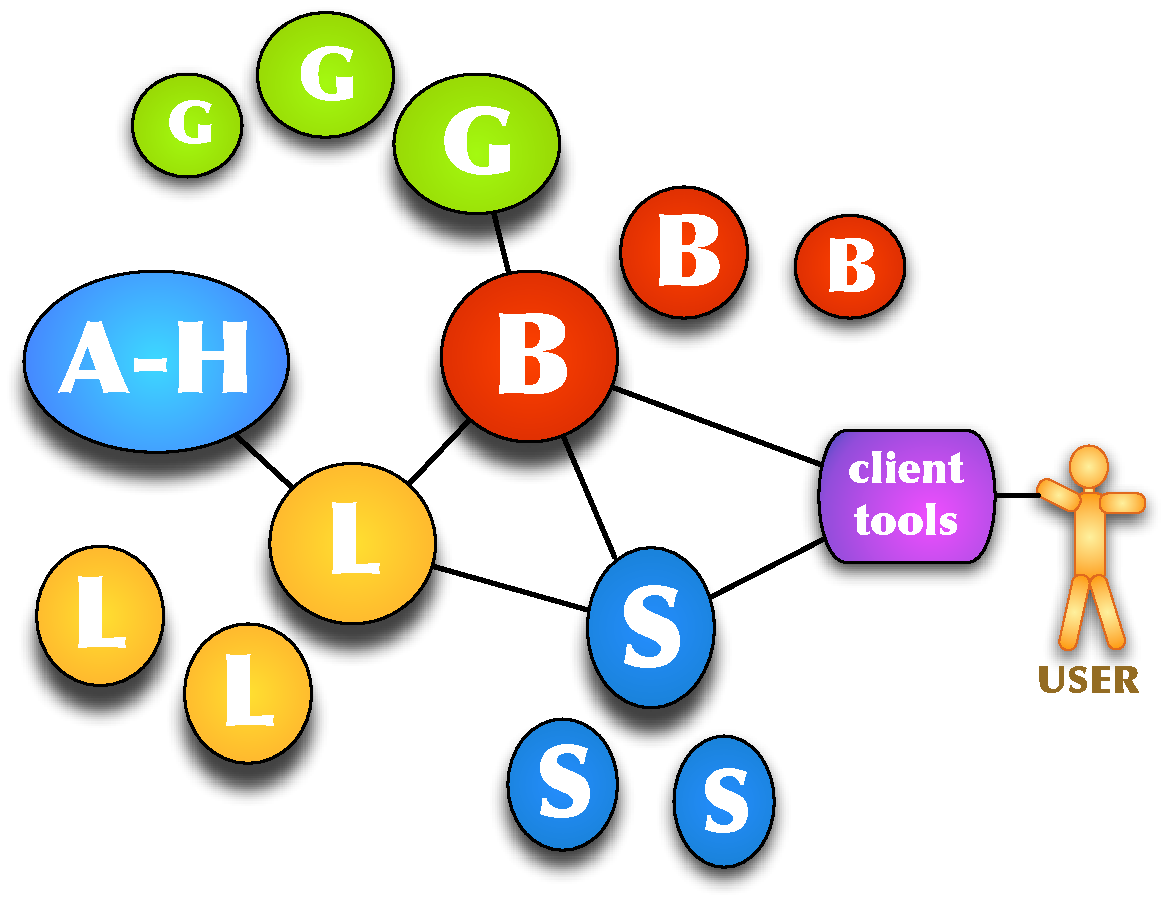
\includegraphics[width=0.8\columnwidth]{arc1-storage-services-with-gateway.pdf}
  \end{center}
  \caption{Schematic of the ARC Storage architecture. The figure shows
    the main services of ARC Storage and the communication channels. The B stands for Bartender, the S Shepherd, the L Librarian, the G Gateway and the A-H stands for A-Hash. The straight lines denote the communication between services.}
  \label{fig:arc1_storage_service}
\end{figure}


Being based on a service-oriented architecture, the ARC
Storage consists of a set of services as shown in Fig.
\ref{fig:arc1_storage_service}. The services are as follows: The Bartender (B)
provides the high-level interface to the user; the Librarian (L)
handles the entire storage namespace, using the A-Hash (A-H) as a metadatabase; the
Gateway (G) provides access to third-party storage systems; and
the Shepherd (S) is the frontend for the physical storage node. 
See Section \ref{Architecture of the ARC Storage} for a detailed
discussion of the different services.   
The services communicate with each other through the
Message Chain Components in HED. The communication channels are
depicted by straight lines in Fig. \ref{fig:arc1_storage_service}.

The system supports file transfer through several transfer protocols,
with client side tools that hide various technical
details such as protocol specification, port numbers
and so on. To provide fault-tolerance, the system implements
automatic file replication, where
the replicas of a file\footnote{In this paper, a file
denotes an entry in the global namespace, while replica denotes the
physical file stored on a storage node.} are always stored on separate
storage nodes\footnote{A
  storage node is a server with a Shepherd, a Shepherd backend
and some storage service.}. To ensure a resilient, self-healing system, the Shepherd
regularly sends heartbeats to one of the Librarians. If the Shepherd fails
to send a heartbeat, one of the Librarians will automatically initiate
re-replication of the replicas between the other Shepherds.

In the default implementation, the services will provide a
full-featured and consistent data storage system using files as an
atomic unit. The scope of the ARC storage system in the forseeable
future is restricted to providing support for file-based data services.
%% there are currently no plans for intrinsic support for database
%% access.

The ARC Storage supports third-party storage services in two
ways. Using the Gateway service, files already stored in some
third-party storage can be accessed using the client tools provided by
the ARC Storage. To make use of third-party services for storing new
files, with the replication and fault-tolerance offered by the ARC
Storage, third-party storage elements can also be used as backends for the
Shepherd service.

External grid middleware components can
access the ARC storage system using ARC data service
interfaces directly. ARC will also provide interface
components that communicate via standard protocols such as SRM, which
will provide a single access point to the whole system.

\section{Architecture of the ARC Storage}
\label{Architecture of the ARC Storage}

In a service-oriented architecture
the role of each service is well defined. Available
objects\footnote{Files, collections, mount points, etc.} in the
system are identified by unique global IDs. These IDs are
categorized according to the object type:

\begin{itemize} 
\item Each  file and collection has a unique ID (GUID).
\item Services are uniquely identified by a serviceID. 
\item The Shepherds in the system identify their files by a referenceID.
\end{itemize} 

Each object in the ARC Storage has a globally
unique ID. A collection contains files and other collections,
and each of these entries has a name unique within the collection very
much like entries in a standard directory on a local filesystem. Besides
files and collections, the ARC Storage has a third type of entry
called mount-points, which are references to the third-party storages
within the global namespace.

Replicas in a distributed storage system can have different states;
they can be broken, deleted, partially uploaded, etc. In the
ARC Storage, all replicas have assigned a state, some of which are
`\textbf{alive}' (if the replica passed the checksum test, and the
Shepherd reports that the storage node is healthy), `\textbf{invalid}'
(if the replica has a wrong checksum, or the Shepherd claims it has no
such replica) and `\textbf{creating}' (if the replica is in
the state of uploading).

In the following, the details of the
architecture are presented in three parts: First we will discuss the
details of the core components, second we will discuss some of the
important features provided by the system, and third we will discuss the security model.

\subsection{Core Components} 
\subsubsection{Bartender}
\label{Bartender}
The Bartender service provides a high-level interface for the storage
system. Clients connect to the Bartender to create and remove
files, collections and mount-points using their Logical Names. The
Bartender communicates 
with the Librarian and Shepherd services to execute the clients'
requests. However, the actual file data does not go through the
Bartender, instead file
transfers are directly performed between the storage nodes and the
clients. There could be any number of independent Bartender services
running in the system, providing high-availability and
load-balancing. 
\subsubsection{Librarian}
\label{librarian}
The Librarian manages the hierarchy and metadata of
files, collections and mount points, as well as the health information of the Shepherd
services. In addition, the Librarian handles
the information about registered Shepherd services. The Librarian receives
heartbeat messages from the Shepherds and changes replica states automatically
if needed. The Librarian uses the A-Hash for consistently storing all metadata. This makes the
Librarian a stateless service, thus enabling the system to have any
number of independent
Librarian services, again providing high-availability in the
system.

\subsubsection{Shepherd}
\label{Shepherd}

The Shepherd services run as front-ends on storage nodes. A Shepherd
service reports to a Librarian about the 
node's health state in terms of replicas. While the Bartender initiates
file transfers, the actual transfers go directly between the Shepherd
and the clients.
 
%% The file-names used by a Shepherd is completely independent from the
%% hierarchy of collections or Logical Names.
When a new replica upload
is initiated, the Shepherd generates a referenceID which refers to
the replica within
that Shepherd. Each Shepherd has a unique serviceID, so with these two
IDs the replica can be unambiguously referenced. This is called a Location
of the replica. %% The namespace of these Locations is independent from
%% the namespace of GUIDs and Logical Names.



\subsubsection{A-Hash}
\label{Hash Algorithm}

A-Hash is a hash table for consistently storing data in property-value
pairs. All metadata about files, collections, mount point, Shepherd's
health status, and so forth, is stored in the A-Hash. As the A-Hash is
the service storing the entire state of the storage system, it is
absolutely crucial for the ARC Storage that the A-Hash is
consistent. The distribution and replication of this service is
therefore both necessary and challenging.

\begin{figure}
\centering
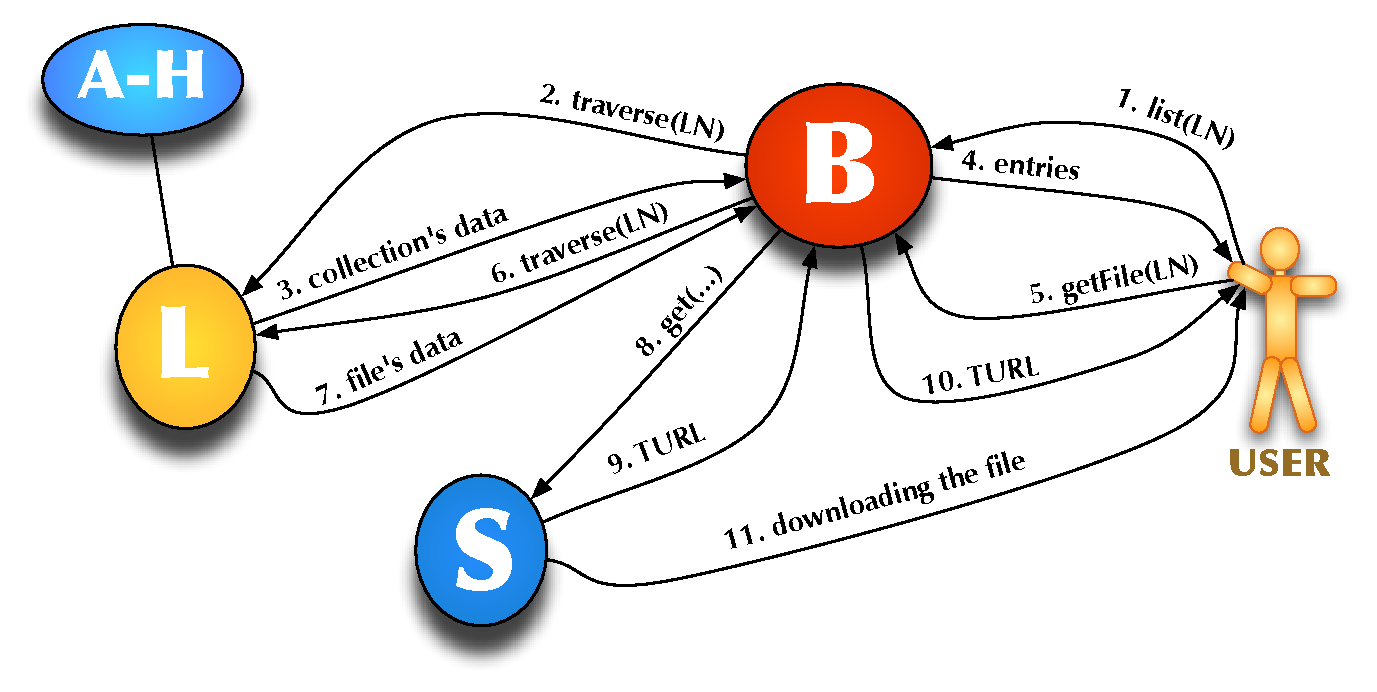
\includegraphics[width=1.0\columnwidth]{arc1-storage-downloading.pdf}
\caption{Schematic showing the scenario of file download from the ARC Storage.}
\label{arc1-storage-downloading}
\end{figure}  


\subsection{Features}
\subsubsection{Heartbeat monitoring}
\label{Heartbeat and Replication}
In the proposed architecture, each Shepherd periodically sends
heartbeats to a Librarian with information about replicas
whose state changed since the last heartbeat, and the corresponding
GUIDs. These heartbeats are then stored in the A-Hash, making them
visible to all the Librarians in the system. If any of the Librarians
notices that a Shepherd is late with its heartbeat, it will invalidate
all the replicas in that Shepherd.  

\subsubsection{Replication}
\label{Replication}
Shepherds periodically ask the Librarian if the file of the replica stored on
its storage node has enough replicas. If the file does not have
enough replicas, the Shepherd informs the Bartender and the Bartender initiates
a put request that returns a Transfer URL to the Shepherd. The
Shepherd finally uploads the new replica. The Shepherd which gets the new replica notifies the
Librarian that the replica is alive. The Librarian then adds this to
the corresponding file.

\subsubsection{Deletion}
\label{Deletion}
In a replicating storage system, there are several possible solutions
for file deletion, since both the replicas and the metadata need to be
removed. In our solution, we use the process of \textit{lazy
  deletion}, \cite{LazyDeletion}. When a client requests that a file
should be deleted (and the user has the proper permissions) the
Bartender instructs the Librarian to remove the file's GUID from the
A-Hash. When the Shepherd, periodically checking all its replicas,
discovers that a replica has no file (and hence, no Location), it will
automatically delete the replica.

\subsubsection{Fault tolerance}
\label{Fault tolerance}

Due to the unpredictable nature of the Grid environment, it is essential to
have some degree of  automatic recovery system in case of unexpected
failures. Fault tolerant behavior is required both at the level of
metadata and on the level of physical storage. While the work on fault-tolerant metadata is still in
progress, the following two
scenarios will explain the currently available recovery mechanism for
physical storage: 
\begin{itemize}
\item In the case of a file having an invalid checksum, the Shepherd
immediately informs the Librarian and the Librarian changes the state of the given replica to
`\textbf{invalid}'. To recover its replica, the Shepherd contacts a
Bartender and asks for another replica of the file. The Bartender chooses a valid
replica, initiates a file transfer from a Shepherd having the replica,
and returns the TURL to the Shepherd with the invalid replica. When the
Shepherd has recieved the replica and compared the checksum, it notifies the
Librarian that the replica is alive again.  
\item In the case of a Shepherd going offline, a Librarian will,
  as mentioned earlier, notice the lack of heartbeats and invalidate all the
  replicas, initiating new replication for all the files stored in
  this storage node. However, if the Shepherd
  again comes online, there will evidently be more replicas than
  needed. The first Shepherd to notice this will set its replica's
  state to `\textbf{thirdwheel}', i.e. obsolete. At the next occasion,
  the Shepherd will remove the replica, if and only if it has the only
  `\textbf{thirdwheel}' replica of this file. If there are more
  replicas with this state, all replicas will be set back to
  `\textbf{alive}' and the process is repeated. This scenario will be discussed further in Section
  \ref{Testing and Discussion}.
\end{itemize}
\subsubsection{Client tools }
\label{Client extension using FUSE module}

Being the only part a user will (and should) see from a storage
system, the client tools are an important part of the ARC
Storage. Currently ARC supports two ways of accessing the
storage solution:
\begin{itemize}
\item The \textbf{Command-line Interface} (CLI) provides
  access to the storage through the methods \texttt{stat}, \texttt{makeCollection},
  \texttt{unmakeCollection}, \texttt{putFile}, \texttt{getFile}, \texttt{delFile},
  \texttt{list} and \texttt{move}. Methods for modifying
  access and ownership will be available in the near future. The CLI
  assumes a relatively high level of computer competence
  from the user. However, the CLI, being a stand-alone tool, can be
  used to access ARC Storage from any computer (also including
  Microsoft Windows PCs) that has network access and
  a Python installation.
\item The \textbf{FUSE module} provides a high-level access to the
  ARC Storage. Filesystem in Userspace (FUSE) \cite{FUSE} provides a simple
  library and a kernel-userspace interface. Using FUSE and the ARC
  Storage Python interface, the FUSE module allows users to mount the
  ARC Storage namespace into the local namespace. This way, the user
  can use her/his favorite file manager to access her/his files and
  collections. The FUSE module provides most of the features provided
  by the CLI, with the exception of modifying some non-posix metadata.
\end{itemize}
It is worth mentioning that the client tools access the storage system
through the Bartender only. Currently upload and download is realized
through HTTP(S), but there are plans to add support for other
protocols, such as SRM and GridFTP.

\subsubsection{Gateways }
\label{Gateways}

Gateways are used to communicate with the external storage
managers. While designing this service, care was taken to: 
\begin{itemize}
\item Retain the transparency of the global namespace while using the external storage systems.
\item  Develop a protocol-oriented  service, i.e. all the external
  storage managers which support a certain protocol should be handled
  using the corresponding gateway service.  
\end{itemize}
This approach provides flexibility while avoiding multiple Gateway
services for different storage managers. Currently, the available
Gateway service is based on the gridftp protocol.  

When the user request is made, the Librarian provides the metadata related
to the request to the Bartender. Requests can be related to
files, collections or external mount-points. In case of creating
external mount-points, the Bartender contacts the Librarian to store
the mount-point for later use. In the case where a request is related
to the downloading of files from the external store, the Gateway service first checks the status of the file
and then sends the Transfer URL (TURL) to the client via the
Bartender. Using this TURL, the client can directly get the file from
the external store. %% For the experiments we use dCache with gridftp
%% protocol as an external storage system.   

\subsection{Security Model }
\label{Security Model }

As is the case for all openly accessible web services, the security
model is of crucial importance for the ARC Storage. The security
architecture of the storage can be split into three parts; the
inter-service authorization; the transfer-level authorization; and the
high-level authorization.
\begin{itemize}
\item The \textbf{inter-service authorization} maintains the integrity of the
  internal communication between services. There is a lot of
  communication between the services of the ARC Storage. The
  Bartenders send requests to the Librarians and the Shepherds, the
  Shepherds communicate with the Librarians and the Librarians talk with
  the A-Hash. If any of these services is compromised or a new
  rogue service gets inserted in the system, the security of the
  entire system is compromised. To enable trust between the services,
  they need to know each other's Distinguished Names (DNs). This way,
  a rogue service would need to obtain a certificate with that exact
  DN from some trusted Certificate Authority (CA).
\item The \textbf{transfer-level authorization} handles the
  authorization in the cases of uploading and downloading files. When
  a transfer is requested, the Shepherd will provide a one-time
  Transfer URL (TURL) to which the client can connect. In the
  current architecture, this TURL is world-accessible. This may not seem
  very secure at first. However, provided that the TURL has a very long,
  unguessable name, that it is transfered to the user in a secure way
  and that it can only be accessed once before it is deleted, the
  chance of being compromized is very low.
\item The \textbf{high-level authorization} considers the access
  policies for the files and collections in the system. These policies
  are stored in A-Hash, in the metadata of the corresponding file or
  collection, providing a fine-grained security in the system.
\end{itemize}
The communication with and within the storage system is realized
through HTTPS with standard X.509 authentication.

\section{Testing and Discussion}
\label{Testing and Discussion}

Even though the ARC Storage is in a pre-prototype state, it is already
possible to deploy and use the system for testing purposes. To
properly run a proof-of-concept test, the resources need to be
geographically distributed. In our test scenarios we utilized
resources in three different countries.

In our test deployment, we used two nodes from Uppsala
Multidisciplinary Center for Advanced Computational Science (UPPMAX), Sweden, 
%each with a 3.00GHz Dual Core Intel(R) Pentium(R) 4 CPU and 4 GB RAM, 
three nodes from the Center for Information Technology (USIT) at the
University of Oslo, Norway, 
%each with two 3.40GHz Dual core Intel(R) Xeon(TM) CPUs with 2GB RAM
and one node from National Information Infrastructure Development Institute (NIIF),
Hungary. %with a 2.00GHz Dual Core Intel(R) Pentium(R) 4 CPU with 4 GB RAM. 

The services were distributed as shown in Fig. \ref{fig:map}:
\begin{itemize}
\item An A-Hash runs at UPPMAX.
\item A Bartender runs at USIT.
\item A Librarian runs at UPPMAX.
\item In total five Shepherds were used for the tests: Three at USIT, having
  100GB storage space each, one at UPPMAX, with 20GB, and one at NIIF, providing 16GB of storage space.
 \end{itemize}

\begin{figure}
\centering
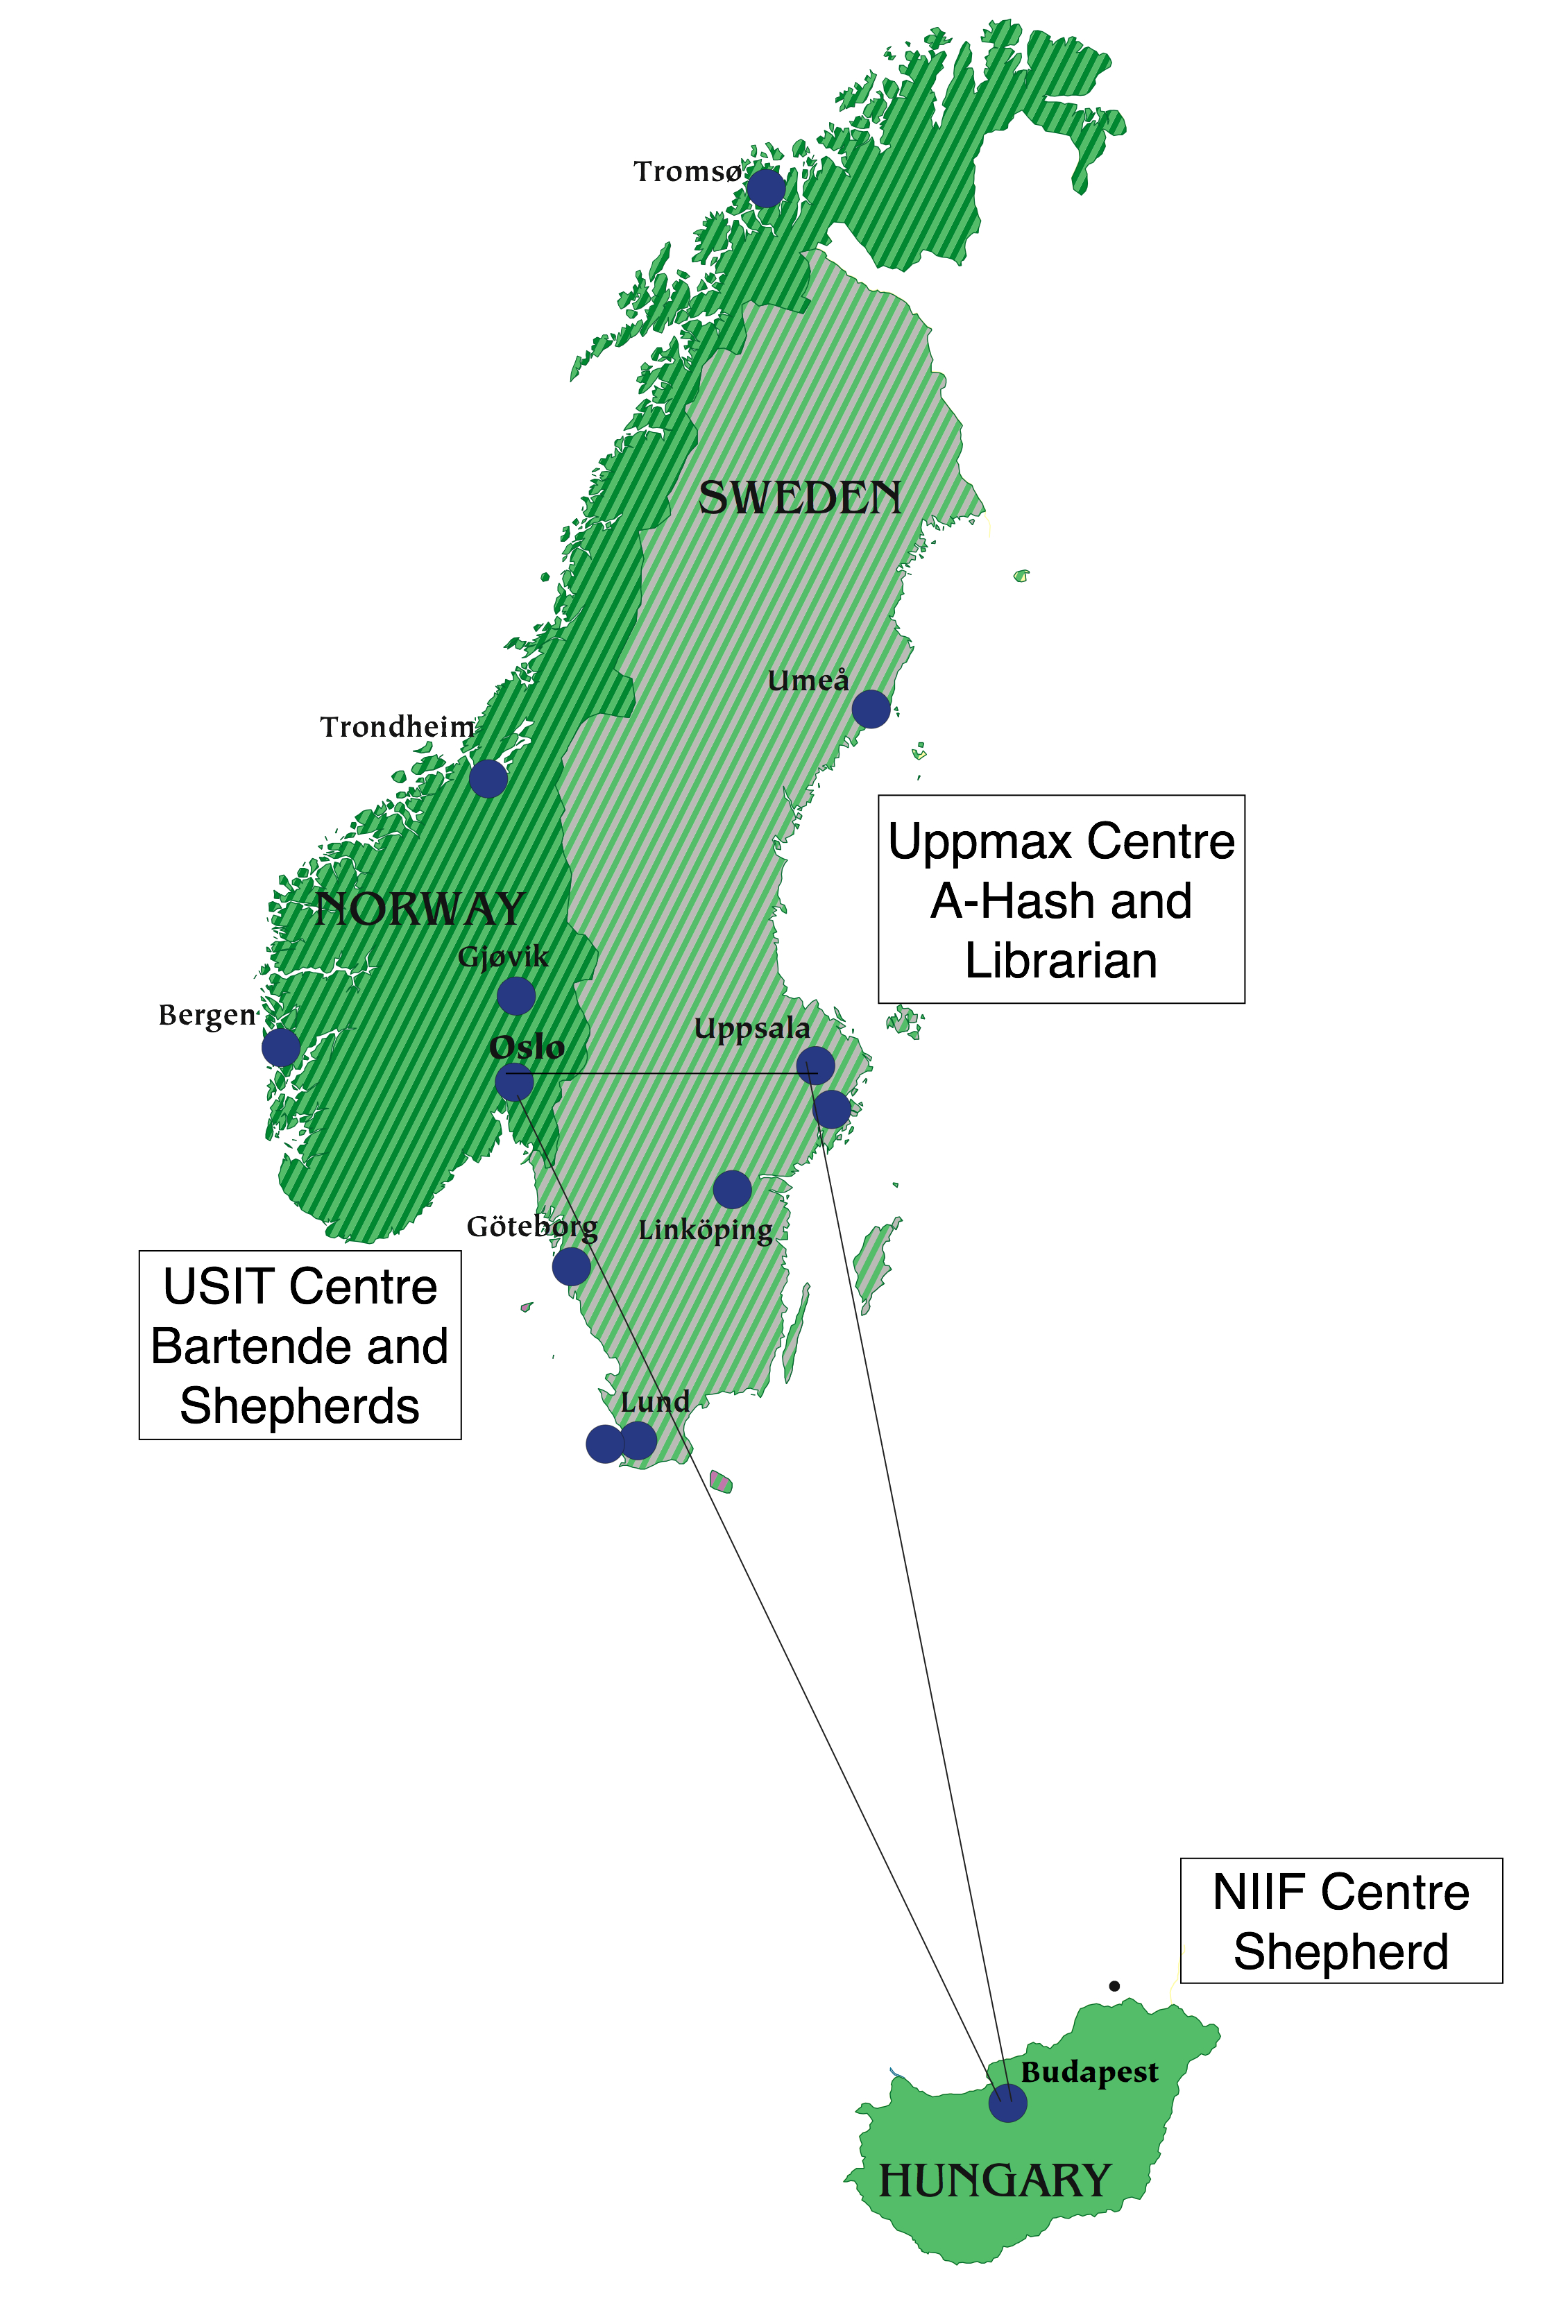
\includegraphics[width=0.7\columnwidth]{map}
\caption{The map shows the geographical distribution of the services in the test setup.}
\label{fig:map}
\end{figure}  

The following tests were carried out:

\begin{itemize}
\item Test 1: The distribution of data after uploading 10 large size (1 GB)
  files with one replica each.  
\item Test 2: The distribution of files after uploading 100 small size (1 kB)
  files with one replica each, and with simultanious uploading.
\item Test 3: The distribution of data after repeating Tests 1 and 2 with three replicas.  
\item Test 4: System behavior while some of the Shepherds are offline.   
\end{itemize}

In the tests we used two client machines: One ASUS eee 901 on a wireless network in Uppsala, 
and one Dell PowerEdge 1425SC with 10Gb ethernet connection at USIT. All the tests were performed and worked as expected: All the files were both 
uploaded and downloaded with correct checksums and they all got the requested 
number of replicas within a reasonable time. However, some of
the tests deserve extra attention.

Fig. \ref{fig:FileDistribution} illustrates two test results,
corresponding to Test 2 and Test 3: The orange (light grey) bars show the distribution after uploading 100 small files
simultaneously, without replication. This gives an indication of how
the system balances the load of many clients uploading at the same
time. The green (dark grey) bars show the distribution with the same kind of
uploading, but with the clients requesting three replicas for each file. The
difference here is that the system simultaneously has to handle both
replication and the clients requesting uploads. When the Bartender chooses
a location for which to put a replica, it generates a list of
Shepherds that (a) do not have a replica of the file, and (b) are not
already in the process of uploading the replica. Next, it draws a
Shepherd from the list at random, using a uniform random number
generator. When uploading without asking for replicas we would
therefore expect a relatively flat distribution of the files, as can
be seen in Fig. \ref{fig:FileDistribution}. 

\begin{figure}
\centering
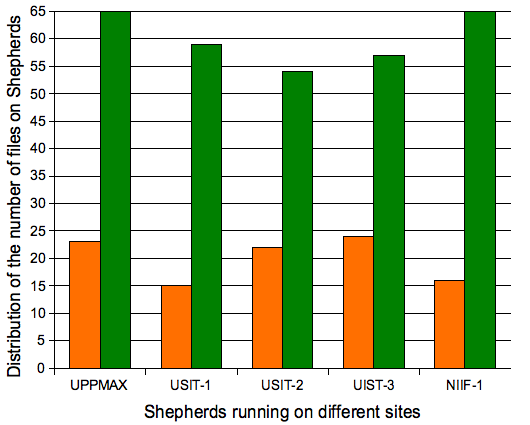
\includegraphics[width=0.8\columnwidth]{FileDistribution}
\caption{The distribution of replicas over the geographically distributed
  storage nodes. Green bars show the distribution in the case where
  we upload 100 files requesting 3 replicas, whereas orange bars show
  the distribution after uploading 100 files without replication. }
\label{fig:FileDistribution}
\end{figure}

\begin{table}[ht]
\centering
%% \begin{tabular}[width = \columnwidth]{p{11mm} p{12mm} p{11mm} p{11mm} p{11mm} p{5mm}}
\begin{tabular}[width = \columnwidth]{llllll}
\hline \hline
&\small{UPPMAX}&\small{USIT-1}&\small{USIT-2}&\small{USIT-3}&\small{NIIF}\\
\hline
           \small{Load(GB)}&6.683&7.638&7.650&4.773&2.289\\
\hline
\end{tabular}
\caption{Overall load distribution on the storage nodes after Tests 1,
2 and 3 were finished}
\label{table:load distribution}  
\end{table}

Table \ref{table:load distribution} shows the disk usage after Tests
1, 2 and 3. It is worth noticing here that the bandwidth to NIIF was
significantly lower than between UPPMAX and USIT. If the bandwidth is
saturated and the storage node is busy, e.g., checksumming a
large file, the heartbeat from this Shepherd may be delayed, causing the
Bartender not to choose this Shepherd for the next replica. This may explain the
relatively low storage load on the  NIIF storage node.

%% \begin{table}[ht]
%% \centering
%% %% \begin{tabular}[width = \columnwidth]{p{11mm} p{12mm} p{11mm} p{11mm} p{11mm} p{5mm}}
%% \begin{tabular}[width = \columnwidth]{llllll}
%% \hline \hline
%% &\small{UPPMAX}&\small{USIT-1}&\small{USIT-2}&\small{USIT-3}&\small{NIIF}\\
%% \hline
%%            \small{Before(GB)}&4.888&7.820&6.843&7.820&3.320\\
%%            \small{During(GB)}&8.798&9.776& - &9.775&2.344 \\
%%            \small{After(GB)}&8.798&6.843&4.888&8.798&1.367\\
%% \hline
%% \end{tabular}
%% \caption{Storage load before, during and after a Shepherd outage.}
%% \label{table:self healing}  
%% \end{table}      

\begin{table}[ht]
\centering
%% \begin{tabular}[width = \columnwidth]{p{11mm} p{12mm} p{11mm} p{11mm} p{11mm} p{5mm}}
\begin{tabular}[width = \columnwidth]{llll}
\hline \hline
&\small{Before (GB)}&\small{During (GB)}&\small{After (GB)}\\
\hline
\small{UPPMAX}&4.888&8.798&8.798\\
\small{USIT-1}&7.820&9.778&6.843\\
\small{USIT-2}&6.843&-    &4.888\\
\small{USIT-3}&7.820&9.774&8.798\\
\small{NIIF}  &3.320&2.344&1.367\\
\hline
\small{Sum}&30.69&30.69&30.69\\
\hline
\end{tabular}
\caption{Storage load before, during and after a Shepherd outage.}
\label{table:self healing}  
\end{table}      

A significant feature of the ARC Storage is its automatic self
healing. Test 4 addresses this feature by studying the effect of
taking one Shepherd out of the system, and later reinserting it. Table
\ref{table:self healing} shows the storage distribution in three
states: Before interrupting a Shepherd, after the USIT-2
Shepherd is interrupted and redistribution of replicas is finished, and
alive, when the Shepherd is restarted and the system again has stabilized. We
can see that all files are properly distributed between the remaining
Shepherds when one of them is disrupted and that the storage load evens out 
again when the Shepherd comes back online. When the
system discovers that there are more replicas than needed, the first
Shepherd noticing will set mark its replica as obsolete. Since the failing Shepherd didn't lose any replicas while
being down, redistribution of replicas is just a matter of deleting
obsolete replicas. We also see that the NIIF node actually got fewer
files when USIT-2 went offline. If two Shepherds simultaneously
start uploading and replicating a missing replica, there will be too many
replicas. Here, a big replica on the NIIF node has randomly been chosen as
obsolete. However, the total storage usage remains the same in all
three cases.

\section{Conclusion and Future Work}
\label{Conclusion and Future Work}

The proposed system is still in an early phase of development, but our test
results demonstrate that the architecture is robust enough to handle
the challenges for distributed large-scale storage. Much
effort is required to make the system production
ready. However, we believe that continuing in the same direction
will enable us to provide a persistent  and flexible storage system
which can fulfill the needs of even the most demanding scientific community. 

Some key areas need special attention and effort to make the proposed
storage system even more stable, reliable and consistent:
\begin{itemize}
\item \textbf{Security:} This is still under development. The design
  is almost ready, but it still needs to be implemented and properly
  tested.
\item \textbf{The A-Hash}: This is currently centralized. To avoid a single
  point of failure in the system, and to improve the system
  performance, the A-Hash needs to be distributed.
\item \textbf{Performance optimization:} To make a storage system
  ready for production, one needs to discover and improve on
  possible bottlenecks within the system. As soon as the A-Hash is
  distributed, other possible bottlenecks, such as load-balancing
  and self-healing mechanisms, will be investigated.
\item \textbf{Protocols:} To ease the interoperability with third-party
  storage solutions and clients, the system needs to support storage
  protocols such as SRM and GridFTP. In addition the system will come
  with its own ARC protocol.
\end{itemize}

%% Even though we have more work in front of us, we have shown that the
%% ARC Storage already is in a state where initial real-life tests can be
%% done. We have described a simple, yet robust architecture which we
%% believe will benefit communities in need of a lightweight,
%% yet distributed storage solution.
While the work in the above mentioned areas is still in progress, we have 
already shown that the ARC Storage already is in a state where initial 
real-life tests can be done. We have described a simple, yet strong 
architecture which we believe will benefit communities in need of a lightweight, 
yet distributed storage solution.

\section{Acknowledgements}
\label{Acknowledgements}

We wish to thank Mattias Ellert for helpful discussions and guidance
on the ARC middleware, to Oxana Smirnova, Alex Read and David Cameron 
for vital comments and proof reading. In addition, we like to thank UPPMAX, NIIF and USIT for
providing resources for running the storage tests.

The work has been supported by the European Commission through the KnowARC
project (contract nr. 032691) and by the Nordunet3 programme through the NGIn
project.

%% In the near future proposed solution will be the part of the ARC
%% middleware production line. We have identified some key areas in which
%% it is essential to put more efforts, to make the system more stable,
%% reliable and consistent. For example: A-Hash is currently centralized
%% and it need to be distributed to avoid single point of failure,
%% require to support more standard protocols like SRM, Better load
%% balancing system for Bartender, more improvements in the self healing
%% mechanism. The work in all these areas is in progress. Hopefully, we
%% will come-up with a reasonably good solutions (One or two last
%% lines)....  
%--------------------------------------------------------
%-----------------------------------------------------------
%% \begin{thebibliography}{5}


%% International Conference on Computing in High Energy and Nuclear Physics (CHEP�07) IOP Publishing 
%% Journal of Physics: Conference Series 119 (2008) 062014 doi:10.1088/1742-6596/119/6/062014 
%% \newline
%% A Simple Mass Storage System for the SRB Data Grid, Michael Wan, Arcot Rajasekar, Reagan Moore, Phil Andrew, 20th IEEE/ 11th NASA Goddard Conference on Mass Storage Systems \& Technologies (MSST2003) San Diego, California, April 7-10, 2003.
%% \newline
%% Advanced Resource Connector middleware for lightweight computational Grids, ELLERT M. ; GRONAGER M. ; KONSTANTINOV A. ; KONYA B. ; LINDEMANN J. ; LIVENSON I. ; NIELSEN J. L. ; NIINIM?KI M. ; SMIRNOVA O. ; WAANANEN A. ;FGCS. Future generations computer systems   ISSN 0167-739X   CODEN FGCSEV

%% \end{thebibliography}

\bibliography{arcstorage_refs}
\bibliographystyle{IEEEtran}

\end{document}
